\documentclass[12pt]{article}

\usepackage{amsmath}
\usepackage[margin = 1in]{geometry}
\usepackage{graphicx}
\usepackage{booktabs}
\usepackage{natbib}
\usepackage[colorlinks=true, citecolor=blue]{hyperref}
\usepackage{underscore}

\title{Using Statistical Modeling to Estimate the Chances of Success of College Basketball Transfers}
\author{Miles Kee}

\begin{document}
\maketitle

\begin{abstract}
When the NCAA decided to eliminate the rule of athletes needing to sit out a season after transferring due to the COVID-19 pandemic, it created a frenzy in the college basketball world. Record numbers of players transferring were seen immediately after this ruling. Since then, the NCAA has decided to make this elimination permanent. This, combined with student athletes newfound ability to profit off their name, image, and likeness, has turned the college basketball offseason into a scene that is more akin to the free agency period in professional sports. Over 1500 players entered the transfer portal during the 2023 offseason. College coaches have began rebuilding their entire teams using the transfer portal instead of the traditional program-building methods of recruiting well and emphasizing player development. For example, new St. John's coach Rick Pitino was hired in March, and by early May, he had already brought in eight new transfers while losing another eight to the transfer portal. This type of roster turnover has become routine in the college game, especially when a coach is fired or hired. 
\end{abstract}

\section{Introduction}
The goal of this project is to use statistical modeling techniques to more efficiently analyze the hundreds, and sometimes thousands, of transfers in the portal. Dean Oliver's "Basketball on Paper" was one of the first pieces of literature that outlined a rating system for basketball players and teams \citep[][]{oliver2004basketball}. It modernized the way people in basketball look at statistics by proposing evaluators normalized to possession counts. Looking at stats on a rate basis, or per a number of possessions (usually 100) allows us to better understand a team's or player's strengths and weaknesses because some teams have more possessions in their games, allowing the team and its players to accumulate counting stats that don't tell the full story of their success or failure, and vice versa with teams that have fewer possessions in their games. \citet{nguyen2022application} looks at using linear regression, classification, and machine learning to predict NBA player performance, using many of the statistics Oliver outlined to train their models. However, not much work has been done in the field of predictive college basketball player ratings. Most of the work in predictive analytics for college basketball involves predicting game outcomes or team ratings, not individual players. \citet{zimmermann2013predicting} uses machine learning to predict the outcomes of games, while \citet{west2006simple} looks at creating a team rating system for predicting success in the college basketball postseason. This project is unique in terms of looking at player ratings, but also due to the novelty of the transfer portal. Very little work has been done on players who enter the transfer portal. \citet{davis2023exploratory} looks at predicting players who will enter the transfer portal, but does not discuss their chances of success afterwards. This study will look to build on the past works by projecting the chances of success of players who enter the transfer portal. The rest of the paper is organized as follows: section~\ref{sec:data} outlines the data sources used and what the data contains. Section~\ref{sec:lms} discusses linear regression techniques used to analyze the players, and section~\ref{sec:cms} looks at classification methods used to analyze the data. Section~\ref{sec:mlnp} uses numerical prediction machine learning techniques to project success and failure of transferring players, while section~\ref{sec:mlc} uses classification machine learning techniques. Section~\ref{sec:results} summarizes the results of analysis, and section~\ref{sec:discussion} discusses the study and what could come next in this field of research.


\section{Data}
\label{sec:data}
The data for this project comes courtesy of \href{barttorvik.com}{barttorvik.com}. The files titled "transferYEAR" contain each player who transferred schools in a given year. For example, the file named "transfer22" contains each transfer that started at their new school during the 2021-2022 season. The rows in each of the transfer files are as follows: player\_name, team, conf, min\_per, ORtg, usg, eFG, ORB\_per, DRB\_per, AST\_per, TO\_per, blk\_per, stl\_per, ftr, yr, ht, new.school, and dbpm. \autoref{tab:data-expl} explains what each of these variables means. \(eFG\) percentage was chosen instead of traditional FG percentage because it properly weighs the added impact of a three pointer when compared to a two pointer by multiplying three pointers made by 1.5. The formula is \(eFG=(2PM+1.5*3PM)/(FGA)\), where \(2PM\) and \(3PM \)are two and three pointers made, respectively, and \(FGA\) is field goals attempted. The offensive statistics in the data are ORtg, usg, eFG, ORB\_per, AST\_per, TO\_per, and ftr. The defensive statistics are DRB\_per, blk\_per, stl\_per, and dbpm. There are many more reliable stats available to track a player's offensive impact when compared to the stats available to track a player's defensive impact. Defense is much more nuanced, as not every good defensive play shows up in a box score. This is why dbpm is used, as it reflects a team's full defensive performance when a player is on the court, allowing us to better quantify an inherently non-quantifiable concept. The data contains files titled "statsYEAR," which are used to look at a player's stats the year after he transferred. The same statistics are used for both the transfer and stats files. Finally, the "fulldata" file contains each transfer from 2021-2023, their stats from the year before they transferred, and their stats from the year after they transferred. The years 2021, 2022, and 2023 are looked at because these are the years the "free agency" aspect of the transfer portal started. The 2024 transfers are excluded from this study because at the time it was conducted, the new season had not given a significant enough sample size to evaluate the players' performances. This leaves us with 2093 players in the "full data" file. The target variables to predict are ORtg and dbpm, as those do the best job of encapsulating a player's impact on offense and defense, respectively, into a single number.
\subsection{Feature Engineering}
\label{subsec:feature-eng}
Once the data was loaded in, I added some features to the data. The variable created called "fromp5" indicates whether a player transferred from a power conference school which in this case are: Big East, Big 12, Big 10, Pac 12, ACC, and SEC. The variable created called "top5" indicates whether a player transferred to a power conference school. The variable called "oimp" indicates whether a player improved their offensive rating from one year to the next year, and the variable called "dimp" indicates the same for a player's dpbm. For all of these created variables, a 1 indicates a "true" value while a 0 indicates a "false" value.


\begin{table}[tbp]
\caption{Variable Explanations}
\centering
\resizebox{\columnwidth}{!}{
\begin{tabular}{@{}ll@{}}
\toprule
Variable & Explanation \\
\midrule
player\_name & The name of the player                                                  \\ 
team         & The team the player played for in the season before he transferred      \\
conf         & The conference the team plays in                                        \\
min\_per     & The percentage of a team's minutes a player played in                   \\
ORtg     & The number of points scored by the player's team per 100 possessions when he was on the court   \\
usg          & The percentage of a team's plays used by the player while on the floor \\
eFG          & A metric to measure a player's shooting success                         \\
ORB\_per     & The percentage of available offensive rebounds a player got             \\
DRB\_per     & The percentage of available defensive rebounds a player got             \\
AST\_per     & The percentage of made shots a player assisted while on the court       \\
TO\_per      & The percentage of turnovers a player committed while on the court       \\
blk\_per & The percentage of opponent shot attempts blocked by a player while on the court                 \\
stl\_per & The percentage of opponent possessions ending in a steal by the player                          \\
ftr          & The number of free throws a player attempts per field goal attempt      \\
yr           & Year in college of the player                                           \\
ht           & Height of the player                                                    \\
new.school   & School the player transferred to                                        \\
dpbm     & The player's defensive contribution in terms of points above league average per 100 possessions \\ 
\bottomrule
\end{tabular}
}
\label{tab:data-expl}
\end{table}

\section{Linear Models}
\label{sec:lms}
To start, I created a correlation matrix of the data, the results of which are shown in \autoref{fig:corrplot}. The first 12 entries in the matrix, from Min\_per to dpbm reference the player's stats from the year before they transferred, while the last 12 correspond to the player's stats from the year after they transferred. The plot shows that defensive metrics are a bit more correlated with each other year to year than offensive metrics. The two variables I am interested in predicting are the player's offensive rating and defensive box plus minus for the year after they transferred. I started by creating a linear model for each, using only offensive and defensive stats, respectively. For the model predicting the next season's offensive rating, the following predictors were used from the previous season: ORtg, eFG, ORB\_per, AST\_per, TO\_per, ftr, fromp5, top5, Min\_per, and usg. For the model predicting the next season's defensive rating, the following predictors were used from the previous season: dpbm, DRB\_per, blk\_per, stl\_per, fromp5, top5, and Min\_per. The data was split into training and testing sets at random, with 70\% of the data being used as a training set and the other 30\% being used for testing. The models for offense and defense are discussed in \ref{subsec:olm} and \ref{subsec:dlm}, respectively. The metric I chose to evaluate the models was mean absolute error, given by 
\begin{equation}
  MAE=\frac{\sum_{i=1}^{n}|x_{i}-p_{i}|}{n},
\end{equation}
where \(x_{i}\) is the actual value, \(p_{i}\) is the predicted value, and \(n\) is the sample size. This metric was chosen because I believed using root mean squared error would give an unfair weight in the error term to observations that had very high errors due to the player simply not playing enough minutes to be able to draw a logical conclusion on.

\begin{figure}[tbp]
	\centering
	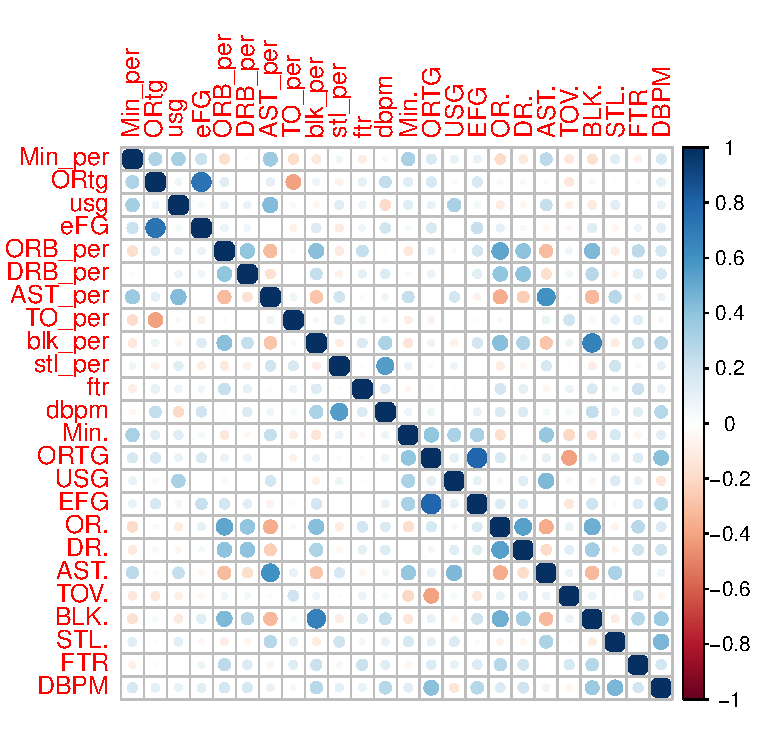
\includegraphics[width=\textwidth]{corrplot}
	\caption{A correlation matrix plot of the variables in the dataset.}
	\label{fig:corrplot}
\end{figure}

\subsection{Offensive Model}
\label{subsec:olm}
In the linear model to predict the next season's offensive efficiency, the statistically significant factors at the .05 significance level were ORtg, ORB\_per, AST\_per, ftr, fromp5, Min_per, and usg. \autoref{fig:olm.test.error} shows the absolute errors on the test set of the model. There were many outliers in this model due to players having very high or low metrics due to playing very little the year before they transferred. The MAE on the test set of this model was 12.53. The model does perform well when predicting whether or not players will improve or not the next year in offensive rating. The model predicted 77.2\% of the players who improved their offensive rating correctly, and 67.4\% of the players who did not improve their offensive rating correctly, for an overall correct prediction rate of 73.2\%. When the model was re-run, but this time only with significant factors from the first running of the model, the MAE was lowered to 12.27. This time, the model correctly predicted 74.0\% of improvements and 70.6\% of non-improvements, for an overall correct rate of 72.6\%. The results of these two models are also shown in \autoref{tab:olm-results}. While the model's MAE is a bit high, it appears to do well when predicting improvements and non-improvements for players. In section~\ref{sec:cms}, I will see if setting the model's goal as classifying improvements and non-improvements helps these metrics.

\begin{figure}[tbp]
	\centering
	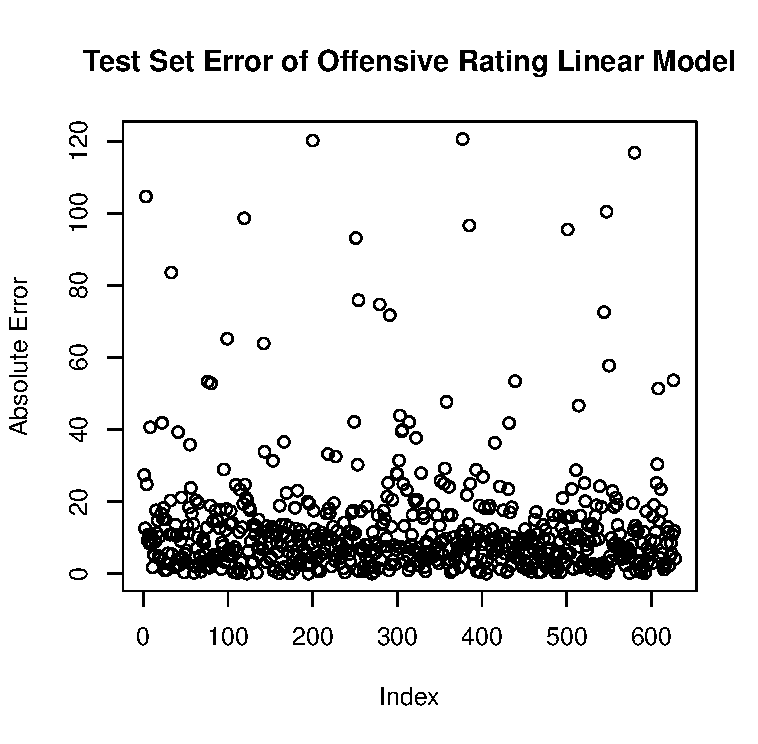
\includegraphics[width=\textwidth]{olm.test.error}
	\caption{A plot of the absolute test set error from the offensive linear model.}
	\label{fig:olm.test.error}
\end{figure}

\begin{table}[tbp]
\caption{Offensive Linear Model Evaluators}
\centering
\resizebox{\textwidth}{!}{
\begin{tabular}{ccccc}
\toprule
Model & MAE & Correct Improvement & Correct Non-improvement & Overall Correct \\
\midrule
First Linear Model & 12.53 & 77.2\% & 67.4\% & 73.2\% \\
Significant Predictors Only & 12.27 & 74.0\% & 70.6\% & 72.6\% \\
\bottomrule
\end{tabular}
}
\label{tab:olm-results}
\end{table}


\subsection{Defensive Model}
\label{subsec:dlm}
In the linear model to predict the following season's defensive box plus minus, the statistically significant factors at the .05 significance level were dbpm, DRB\_per, blk\_per, fromp5, top5, and Min\_per. \autoref{fig:dlm.test.error} shows the absolute errors on the test set for this model. Similarly to the offensive model, there were some outliers due to players having very little playing time. The MAE on the test set of this model was 1.22. Since dbpm is read on a different scale than ORtg, it is not possible to compare the MAE's of the models to determine which is easier to predict, although I will compare the MAE's of different types of models for offense and defense. In terms of predicting improvement, this model correctly predicted 75.6\% and 72.7\% of improvements and non-improvements, respectively. The overall correct prediction rate for this model was 74.2\%. Defensive improvement is a bit more inconsistent than offensive improvement, as it is less of a certainty for a player to improve their defensive traits year over year than their offensive ones. This means in theory, predicting defensive improvement is a bit more difficult, but this model actually predicted it at a similar rate as the offensive model did. When the model was re-run to only include significant factors, the MAE on the test set remains 1.22. The classification rates of this model were 76.3\% for improvements and 73.1\% for non-improvements, for an overall rate of 74.7\%. The summary of these results are also shown in \autoref{tab:dlm-results}.


\begin{figure}[tbp]
	\centering
	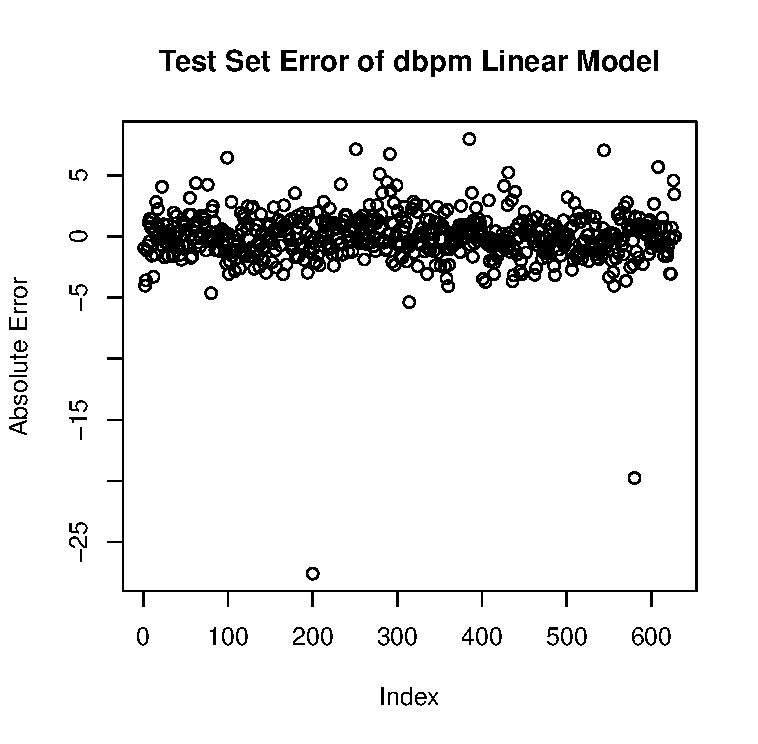
\includegraphics[width=\textwidth]{dlm.test.error}
	\caption{A plot of the absolute test set error from the defensive linear model.}
	\label{fig:dlm.test.error}
\end{figure}

\begin{table}[tbp]
\caption{Defensive Linear Model Evaluators}
\centering
\resizebox{\textwidth}{!}{
\begin{tabular}{ccccc}
\toprule
Model & MAE & Correct Improvement & Correct Non-improvement & Overall Correct \\
\midrule
First Linear Model & 1.22 & 75.6\% & 72.7\% & 74.2\% \\
Significant Predictors Only & 1.22 & 76.3\% & 73.1\% & 74.7\% \\
\bottomrule
\end{tabular}
}
\label{tab:dlm-results}
\end{table}


\section{Classification Models}
\label{sec:cms}
Since the linear models performed better when attempting to classify improvements and non-improvements, I next moved on to creating a model based solely on classifying these two outcomes. A similar style using logistic regression was followed for each model as in section~\ref{sec:lms}, where offensive and defensive improvement were examined separately. Again, 70\% of the data was used for a training the model and the other 30\% was used for testing. While the MAE does not technically exist for logistic models, there is a very similar metric known as the Brier Score \citep[][]{rufibach2010use}. The Brier Score is given by 
\begin{equation}
  BS=\frac{1}{n}\sum_{i=1}^{n}(x_{i}-p_{i})^{2},
\end{equation}
where \(x_{i}\) is the actual 1 or 0 indicating improvement or lack thereof, \(p_{i}\) is the probability given by the model of improvement, and \(n\) is the sample size. I used this metric on the test set in place of MAE for the classification models. While the Brier Score will not be on the same scale as the MAE of the linear models since it is comparing probability differences, it is now possible to compare the offensive and defensive models on the same scale.

\subsection{Offensive Model}
\label{subsec:ocm}
The statistically significant factors in the logistic model trying to predict offensive improvement were ORtg, TO\_per, fromp5, Min\per, and usg. When compared to the significant factors from the  linear model, ORB\_per and AST\_per were no longer significant, while TO\_per becomes significant. The Brier Score of this model was 0.19. The model correctly predicted 80.7\% of improvements, yet it only correctly predicted 60.0\% of non-improvements. The overall successful prediction rate of this model was 72.1\%, so even though the improvement and non-improvement percentages fluctuated, the overall correct percentage remained about the same as in the linear models. When only significant factors were used in the model, the Brier Score slightly increases to 0.19. The successful improvement prediction rate becomes 78.8\%, and the successful non-improvement prediction rate becomes 63.1\%. The overall correct prediction rate of this model was increased to 72.3\%. Finally, when the model was re-run with the same factors used in the final linear regression model, which were ORtg, ORB\_per, AST\_per, ftr, fromp5, Min_per, and usg, the Brier Score was 0.19. This model was able to successfully predict 80.7\% of improvements and 61.2\% of non-improvements. Overall, the correct prediction rate for this model was 72.6\%. The results of these models are summarized in \autoref{tab:ocm-results}.

\begin{table}[tbp]
\caption{Offensive Classification Model Evaluators}
\centering
\resizebox{\textwidth}{!}{
\begin{tabular}{ccccc}
\toprule
Model & Brier Score & Correct Improvement & Correct Non-improvement & Overall Correct \\
\midrule
First Classification Model & 0.19 & 80.7\% & 60.0\% & 72.1\% \\
Significant Predictors Only & 0.19 & 78.8\% & 63.1\% & 72.3\% \\
Same Predictors as Significant in Linear Model & 0.19 & 80.7\% & 61.2\% & 72.6\% \\
\bottomrule
\end{tabular}
}
\label{tab:ocm-results}
\end{table}


\subsection{Defensive Model}
\label{subsec:dcm}
In the logistic model to predict defensive improvement, dbpm, DRB\_per, blk\_per, stl\_per, fromp5, top5, and Min\_per were significant. In comparison to the linear defensive model, the only change was that stl\_per became significant. All of the defensive predictors used were statistically significant in this model, so the model only using significant predictors is the same as the model using all the predictors. The Brier Score of this model was 0.18, which was slightly better than any of the offensive classification models. The model correctly predicted 76.6\% of improvements in dbpm and 71.1\% of non-improvements. Overall, this model correctly predicted 73.9\% of the improvements and non-improvements correctly, which was again slightly better than the offensive classification models. When I modified the model to include the same parameters that were found significant in the linear defensive model, the Brier Score remains 0.18. Now, the model correctly predicted 79.1\% of defensive improvements. The non-improvement prediction rate lowered to 68.8\%, and the overall successful prediction rate increased slightly to 74.0\%. These results are also summarized in \autoref{tab:dcm-results}.

\begin{table}[tbp]
\caption{Offensive Classification Model Evaluators}
\centering
\resizebox{\textwidth}{!}{
\begin{tabular}{ccccc}
\toprule
Model & Brier Score & Correct Improvement & Correct Non-improvement & Overall Correct \\
\midrule
First Classification Model & 0.18 & 76.6\% & 71.1\% & 73.9\% \\
Significant Predictors Only & 0.18 & 76.6\% & 71.1\% & 73.9\% \\
Same Predictors as Significant in Linear Model & 0.18 & 79.1\% & 68.8\% & 74.0\% \\
\bottomrule
\end{tabular}
}
\label{tab:dcm-results}
\end{table}

\section{Machine Learning Numerical Prediction Models}
\label{sec:mlnp}
Next, I moved on to attempting to predict transfer success using machine learning techniques, specifically neural networks. The same training and testing split was used as in the linear and logistic models. For both offensive and defensive models, one hidden layer, a batch size of 50, the ReLU activation function, and an epoch length of 300 were used to fit the model. RMSprop, which is an improved version of gradient descent, was used as the optimizer when compiling the model. More information about the RMSprop optimizer can be found from \citet{rmsprop}. The layer sizes of the neural networks varied a bit due to the different number of predictors used in the offensive and defensive models. \citet{hunter2012selection} proposes that the best number of neurons to use in a one hidden layer neural network is \(n = N + 1\), where \(N\) is equal to the number of inputs. With an output layer of one neuron, it is then suggested that \(N\) neurons are used in the hidden layer, which was the strategy I chose to follow. For both models, the loss function used was MSE. The same metrics as used for the linear regression models were used for the machine learning models.

\subsection{Offensive Model}
\label{subsec:omlnp}
For the offensive model, all predictors were used. These predictors were ORtg, eFG, ORB\_per, AST\_per, TO\_per, ftr, fromp5, top5, Min\_per, and usg. Following the strategy outlined in section~\ref{sec:mlnp}, 11 neurons were used in the hidden layer of the model. \autoref{fig:omlnp.test.error} shows the absolute error on the test set of the model. The model has an MAE of 9.93 on the test set. This model was excellent in terms of classification. It successfully predicted 97.6\% of improvements as well as 97.6\% of non-improvements, for an overall rate of 97.6\%. So, while the MAE, was comparable to the linear offensive model, this model does a much better job of classifying players. These results are summarized in \autoref{tab:omlnp-results}.

\begin{figure}[tbp]
	\centering
	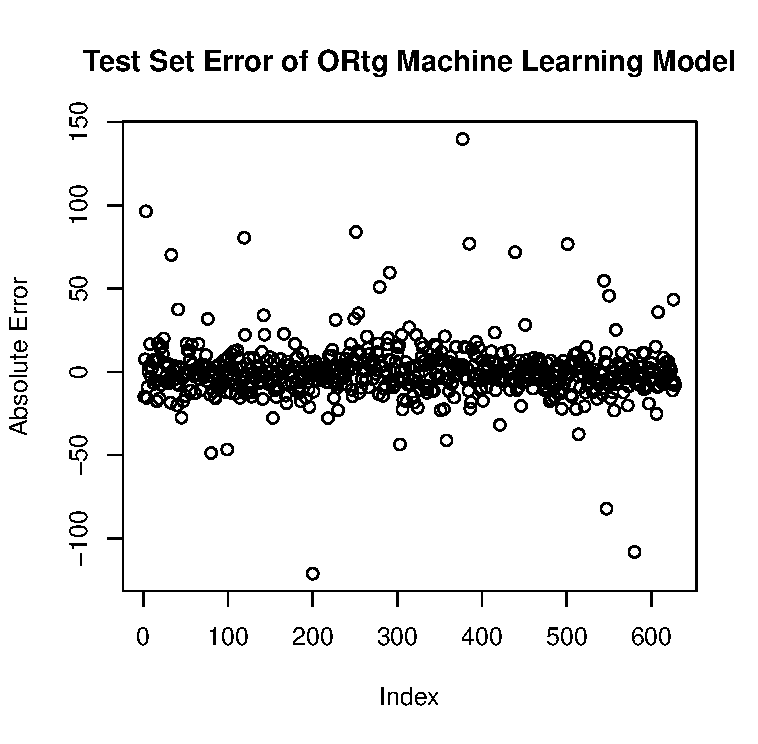
\includegraphics[width=\textwidth]{omlnp.test.error}
	\caption{A plot of the absolute test set error from the offensive machine learning model.}
	\label{fig:omlnp.test.error}
\end{figure}

\begin{table}[tbp]
\caption{Offensive Neural Network Model Evaluators}
\centering
\resizebox{\textwidth}{!}{
\begin{tabular}{ccccc}
\toprule
Model & MAE & Correct Improvement & Correct Non-improvement & Overall Correct \\
\midrule
Neural Network Model & 9.93 & 97.6\% & 97.6\% & 97.6\% \\
\bottomrule
\end{tabular}
}
\label{tab:omlnp-results}
\end{table}

\subsection{Defensive Model}
\label{subsec:dmlnp}
Similar to the offensive model, all available predictors were used. These predictors were dbpm, DRB\_per, blk\_per, stl\_per, Min\_per, fromp5, and top5. Again, following the same strategy outlined in section~\ref{sec:mlnp}, 7 neurons were used in the hidden layer. The absolute error on the test set is shown in \autoref{fig:dmlnp.test.error}. This model performed  closely to the previous defensive model. It had a MAE of 1.34. It successfully predicted 76.9\% of improvements and 70.1\% of non-improvements for an overall correct prediction rate of 73.6\%.  The results are summarized in \autoref{tab:dmlnp-results}.

\begin{figure}[tbp]
	\centering
	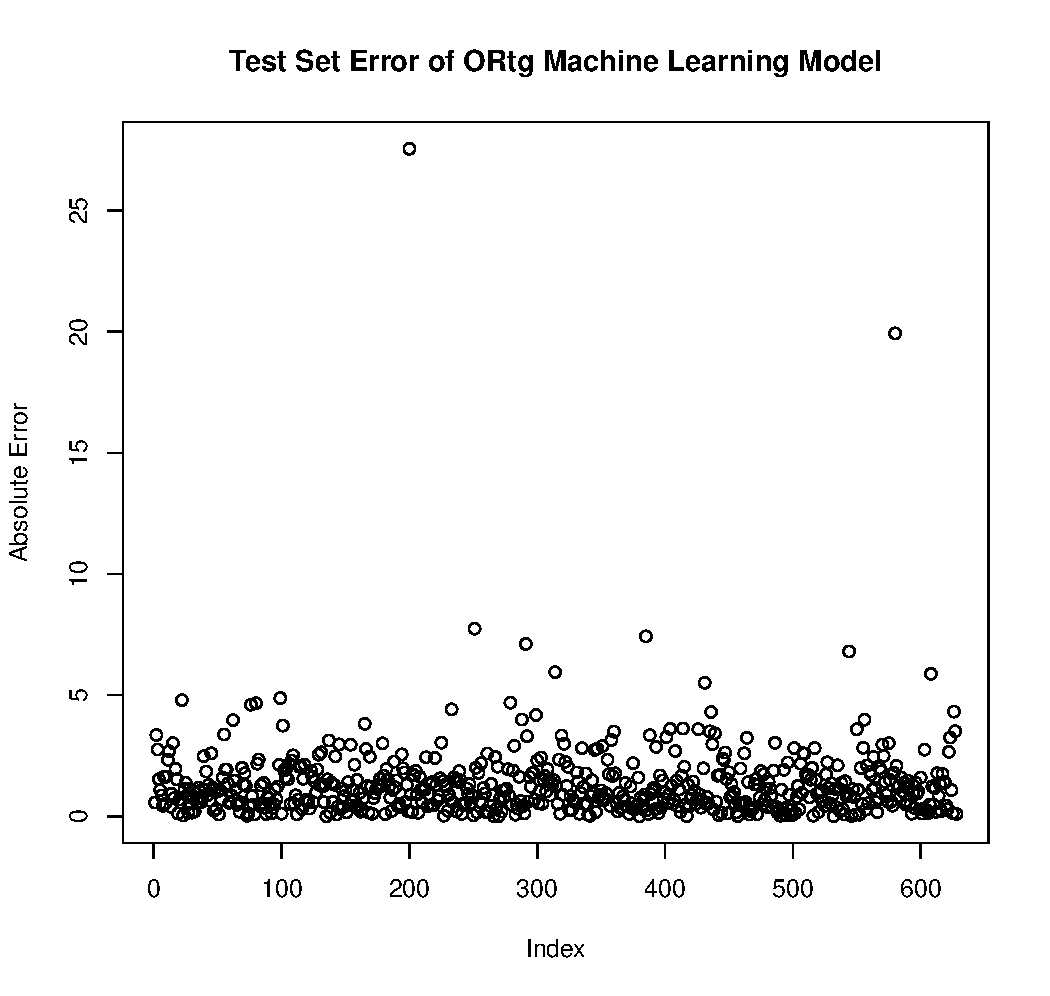
\includegraphics[width=\textwidth]{dmlnp.test.error}
	\caption{A plot of the absolute test set error from the defensive machine learning model.}
	\label{fig:dmlnp.test.error}
\end{figure}

\begin{table}[tbp]
\caption{Defensive Neural Network Model Evaluators}
\centering
\resizebox{\textwidth}{!}{
\begin{tabular}{ccccc}
\toprule
Model & MAE & Correct Improvement & Correct Non-improvement & Overall Correct \\
\midrule
Neural Network Model & 1.34 & 76.9\% & 70.1\% & 73.6\% \\
\bottomrule
\end{tabular}
}
\label{tab:dmlnp-results}
\end{table}

\section{Machine Learning Classification Models}
\label{sec:mlc}
The process of building a classification neural network is very similar to one for numerical prediction, with a few changes. Since the output layer will have two neurons because binary classification was used, these models will have \(n=N+2\) neurons. I made the choice to change to this strategy in order to keep the number of neurons in the hidden layer consistent so the models were more comparable. In this case, for the output layer, the sigmoid (or logistic) activation function was used. The loss function used in this case was binary cross entropy, which is considered the best loss function to use for classification tasks \citep[][]{ruby2020binary}. For consistency, the same batch size and epoch length were used for these models. Brier Score was once again used to evaluate these classification models.

\subsection{Offensive Model}
\label{subsec:omlc}
For this offensive model, again all predictors were used. These predictors were ORtg, eFG, ORB\_per, AST\_per, TO\_per, ftr, fromp5, top5, Min\_per, and usg. 11 neurons were once again used in the hidden layer. This model had a Brier Score of 0.36. It correctly predicted 80.7\% of offensive improvements and 61.2\% of defensive improvements. The overall successful prediction rate the model was 72.6\%. The results are summarized in \autoref{tab:omlc-results}.

\begin{table}[tbp]
\caption{Offensive Neural Network Classification Model Evaluators}
\centering
\resizebox{\textwidth}{!}{
\begin{tabular}{ccccc}
\toprule
Model & Brier Score & Correct Improvement & Correct Non-improvement & Overall Correct \\
\midrule
Neural Network Classification Model & 0.36 & 80.7\% & 61.2\% & 72.6\% \\
\bottomrule
\end{tabular}
}
\label{tab:omlc-results}
\end{table}

\subsection{Defensive Model}
\label{subsec:dmlc}
For the defensive model, all predictors were once again used. These predictors were dbpm, DRB\_per, blk\_per, stl\_per, Min\_per, fromp5, and top5. I used 7 neurons in the hidden layer. This model's Brier Score was 0.35. It predicted 78.1\% of defensive improvements and 69.5\% of defensive non-improvements. The overall correct prediction rate was 73.9\%. The results of this model are summarized in \autoref{tab:dmlc-results}. 

\begin{table}[tbp]
\caption{Defensive Neural Network Classification Model Evaluators}
\centering
\resizebox{\textwidth}{!}{
\begin{tabular}{ccccc}
\toprule
Model & Brier Score & Correct Improvement & Correct Non-improvement & Overall Correct \\
\midrule
Neural Network Classification Model & 0.35 & 78.1\% & 69.5\% & 73.9\% \\
\bottomrule
\end{tabular}
}
\label{tab:dmlc-results}
\end{table}

\section{Summary of Results}
\label{sec:results}
\autoref{tab:fullresults} shows the results of all models with their error metric (MAE or Brier Score), successful prediction rate for improvements and non-improvements, and overall successful prediction rate.

\begin{table}[tbp]
\caption{Model Evaluation Summary}
\centering
\resizebox{\textwidth}{!}{
\begin{tabular}{ccccc}
\toprule
\textbf{Model} & \textbf{Error Metric} & \textbf{Correct Improvement} & \textbf{Correct Non-improvement} & \textbf{Overall Correct} \\
\midrule
\textbf{Offensive Models} & & & & \\
\textbf{Numerical Prediction Models} & \textbf{MAE} & & & \\
First Linear Model & 12.53 & 77.2\% & 67.4\% & 73.2\% \\
Linear Model with Significant Predictors Only & 12.27 & 74.0\% & 70.6\% & 72.6\% \\
Neural Network Model & 9.93 & 97.6\% & 97.6\% & 97.6\% \\
\textbf{Classification Models} & \textbf{Brier Score} & & & \\
First Logistic Model & 0.19 & 80.7\% & 60.0\% & 72.1\% \\
Logistic Model with Significant Predictors Only & 0.19 & 78.8\% & 63.1\% & 72.3\% \\
Same Predictors as Significant in Linear Model & 0.19 & 80.7\% & 61.2\% & 72.6\% \\
Neural Network Classification Model & 0.36 & 80.7\% & 61.2\% & 72.6\% \\
\textbf{Defensive Models} & & & & \\
\textbf{Numerical Prediction Models} & \textbf{MAE} & & & \\
First Linear Model & 1.22 & 75.6\% & 72.7\% & 74.2\% \\
Significant Predictors Only & 1.22 & 76.3\% & 73.1\% & 74.7\% \\
Neural Network Model & 1.34 & 76.9\% & 70.1\% & 73.6\% \\
\textbf{Classification Models} & \textbf{Brier Score} & & & \\
First Logistic Model & 0.18 & 76.6\% & 71.1\% & 73.9\% \\
Logistic Model with Significant Predictors Only & 0.18 & 76.6\% & 71.1\% & 73.9\% \\
Same Predictors as Significant in Linear Model & 0.18 & 79.1\% & 68.8\% & 74.0\% \\
Neural Network Classification Model & 0.35 & 78.1\% & 69.5\% & 73.9\% \\
\bottomrule
\end{tabular}
}
\label{tab:fullresults}
\end{table}

\subsection{Offensive Models}
\label{subsec:off-results}
\subsubsection{Numerical Prediction Models}
\label{subsubsec:npoff-results}
For the numerical prediction models, the neural network model performed by far the best. It had the lowest MAE, and successfully predicted 97.6\% of the outcomes. This was over 20\% higher than any of the other models. Outside of the neural network model, the first linear model and the linear model with significant predictors had very similar MAEs and improvement prediction rates. The first model was a bit better at predicting improvements, while the one with significant predictors only was better at predicting non-improvements. The first linear model had a higher overall prediction rate by 0.6\%. It could be argued, however, that the model with only significant predictors was a better model due to its simplicity and very comparable performance to the more complex one. 
\subsubsection{Classification Models}
\label{subsubsec:classoff-results}
The three logistic models all had similar Brier Scores, and the neural network model had a much higher Brier Score than all three. However, the models were remarkably similar in terms of prediction rate. The first logistic model, the logistic model with the predictors that were significant in the linear model, and the neural network model were tied for the best improvement prediction rate. None of these models were great at predicting non-improvements, but the logistic model using significant predictors only had the best rate of the three. Overall, the logistic model using the predictors significant in the linear model and the neural network model had the best prediction rates. Of these four models, I would say the best one was the logistic model using the same predictors that were significant in the linear model due to its relative simplicity and low Brier Score combined with high prediction rates. 
\subsubsection{Overall Comparison}
\label{subsubsec:ovroff-results}
Of the seven models made to predict the next season's offensive efficiency, the numerical prediction neural network model performed the best. It had the highest prediction rate for all three categories, and the lowest MAE of the numerical prediction models. In the full dataset, 56.3\% of players improved the following year offensively, and 43.7\% did not. So, all of the models made performed admirably when compared to basic guessing or other baseline models that could have been made. Each model predicted a higher improvement rate and a higher non-improvement rate than the dataset would have indicated.
\subsection{Defensive Models}
\label{subsec:def-results}
\subsubsection{Numerical Prediction Models}
\label{subsubsec:npdef-results}
For the numerical prediction models, the two linear models had the lowest MAE's, with the neural network model having the highest MAE. The neural network model was able to correctly predict improvement rates at the highest rate, while the linear model using only significant predictors had the highest rate of correct non-improvements. Overall, the linear model also had the highest correct prediction rate. I would say the linear model with significant predictors performed the best of the three, since it had the highest overall correct rate and performed well in both categories of prediction. It was also the simplest model of the three and was tied for the lowest MAE. 
\subsubsection{Classification Models}
\label{subsubsec:classdef-results}
Of the classification models, the neural network model had the highest Brier Score, while the other three were tied in Brier Score. The logistic model using the same predictors that were significant in the linear model had the highest correct improvement prediction rate. The first logistic model and the logistic model using only significant predictors were tied for the highest correct non-improvement rate. The logistic model using the same predictors that were significant in the linear model had the highest overall correct prediction rate, but all four rates were very similar. Declaring which model is the best of these is a bit more difficult than for the other model types. Since they all had very similar correct prediction rates, model simplicity would likely be the best way to categorize the best model. However, the logistic model using only significant predictors from the logistic regression and the logistic model using the same significant predictors from the linear model are very similar in terms of simplicity. The choice of model would then come down to whether you value predicting improvements or non-improvements more, as the logistic model using only significant predictors from the logistic regression predicted non-improvements better, but the logistic model using the same significant predictors from the linear model predicted improvements better.
\subsubsection{Overall Comparison}
\label{subsubsec:ovrdef-results}
Of the seven models made for defensive prediction, the linear regression model using significant predictors only had the highest correct prediction rate. Due to its relative simplicity and good performance in all metrics, I would say that model was the best of the seven. In the full dataset, 51.6\% of players improved on defense the following year, while 48.4\% did not. This is much more of an even split than what was seen offensively, so for the defensive models to predict improvements and non-improvements correctly at a similar rate to the offensive models (for the most part) is impressive.
\subsection{Model Selection}
The models chosen as the best depend on a few different things. If you valued consistency of model type for offense and defense, the first linear model approach would likely be selected, as it performed comparably to the others in terms of MAE and was second best in terms of prediction rate for both categories. If you valued highest prediction rate, then the neural network model would be selected for offense and the linear model with significant predictors only would be chosen for defense. If you valued lowest MAE or Brier Score when compared to others in its category, you would likely choose one of the logistic models. Interestingly, the numerical prediction models performed better in prediction rate essentially across the board when compared to the classification models. Even though the objective of the classification models was to predict improvements and non-improvements, it seems that a better approach is to predict offensive rating or defensive box plus minus and then see whether that was an improvement or a non-improvement.

\section{Discussion}
\label{sec:discussion}
All of the models were able to correctly classify at an overall rate greater than 70\%. In the dataset, improvement and non-improvement was quite ambiguous, as for both offense and defense players were split fairly evenly in terms of improvement and non-improvement, so to be able to project their success at a rate over 70\% is quite impressive. Teams could use this to identify players to look further into or avoid based off their projected improvement or lack thereof. Coaches and support staff could then evaluate targeted players on their own, but use the model's help to identify their targets. While the models work very well for classification, their are some limitations in terms of prediction. The distinction between a good and bad offensive efficiency is very small, as a difference in five rating points can change an offensive rating from above to below average. Due to this small window, more reliable numerical prediction is likely needed before models are used to explicitly predict a player's efficiency. College basketball is inherently unpredictable, which is one of the qualities of the sport that its fans love. 18-22 year olds are, in general, a very unpredictable group, and this combined with all of the non-basketball factors that go into a college basketball player's performance can make the sport very hard to model. In the future, being able to quantify factors like a player's fit within their team's offensive or defensive system or a coach's ability to motivate their players would be able to make these models significantly better.


\bibliography{workcited}
\bibliographystyle{plainnat}

\end{document}